%%%%%%%%%%%%%%%%%%%%%%%%%%%%%%%%%%%%%%%
% Deedy - One Page Two Column Resume
% LaTeX Template
% Version 1.1 (30/4/2014)
%
% Original author:
% Debarghya Das (http://debarghyadas.com)
%
% Original repository:
% https://github.com/deedydas/Deedy-Resume
%
% IMPORTANT: THIS TEMPLATE NEEDS TO BE COMPILED WITH XeLaTeX
%
% This template uses several fonts not included with Windows/Linux by
% default. If you get compilation errors saying a font is missing, find the line
% on which the font is used and either change it to a font included with your
% operating system or comment the line out to use the default font.
% 
%%%%%%%%%%%%%%%%%%%%%%%%%%%%%%%%%%%%%%
% 
% TODO:
% 1. Integrate biber/bibtex for article citation under publications.
% 2. Figure out a smoother way for the document to flow onto the next page.
% 3. Add styling information for a "Projects/Hacks" section.
% 4. Add location/address information
% 5. Merge OpenFont and MacFonts as a single sty with options.
% 
%%%%%%%%%%%%%%%%%%%%%%%%%%%%%%%%%%%%%%
%
% CHANGELOG:
% v1.1:
% 1. Fixed several compilation bugs with \renewcommand
% 2. Got Open-source fonts (Windows/Linux support)
% 3. Added Last Updated
% 4. Move Title styling into .sty
% 5. Commented .sty file.
%
%%%%%%%%%%%%%%%%%%%%%%%%%%%%%%%%%%%%%%%
%
% Known Issues:
% 1. Overflows onto second page if any column's contents are more than the
% vertical limit
% 2. Hacky space on the first bullet point on the second column.
%
%%%%%%%%%%%%%%%%%%%%%%%%%%%%%%%%%%%%%%

\documentclass[]{deedy-resume-openfont}


\begin{document}

%%%%%%%%%%%%%%%%%%%%%%%%%%%%%%%%%%%%%%
%
%     LAST UPDATED DATE
%
%%%%%%%%%%%%%%%%%%%%%%%%%%%%%%%%%%%%%%


%%%%%%%%%%%%%%%%%%%%%%%%%%%%%%%%%%%%%%
%
%     TITLE NAME
%
%%%%%%%%%%%%%%%%%%%%%%%%%%%%%%%%%%%%%%


\namesection{Nicola}{Borghi}{{\LARGE Ingénieur système - Ingénieur d'essai}}

%%%%%%%%%%%%%%%%%%%%%%%%%%%%%%%%%%%%%%
%
%     COLUMN ONE
%
%%%%%%%%%%%%%%%%%%%%%%%%%%%%%%%%%%%%%%

\begin{minipage}[t]{0.37\textwidth} 

%%%%%%%%%%%%%%%%%%%%%%%%%%%%%%%%%%%%%%
%     LINKS
%%%%%%%%%%%%%%%%%%%%%%%%%%%%%%%%%%%%%%

\section{}
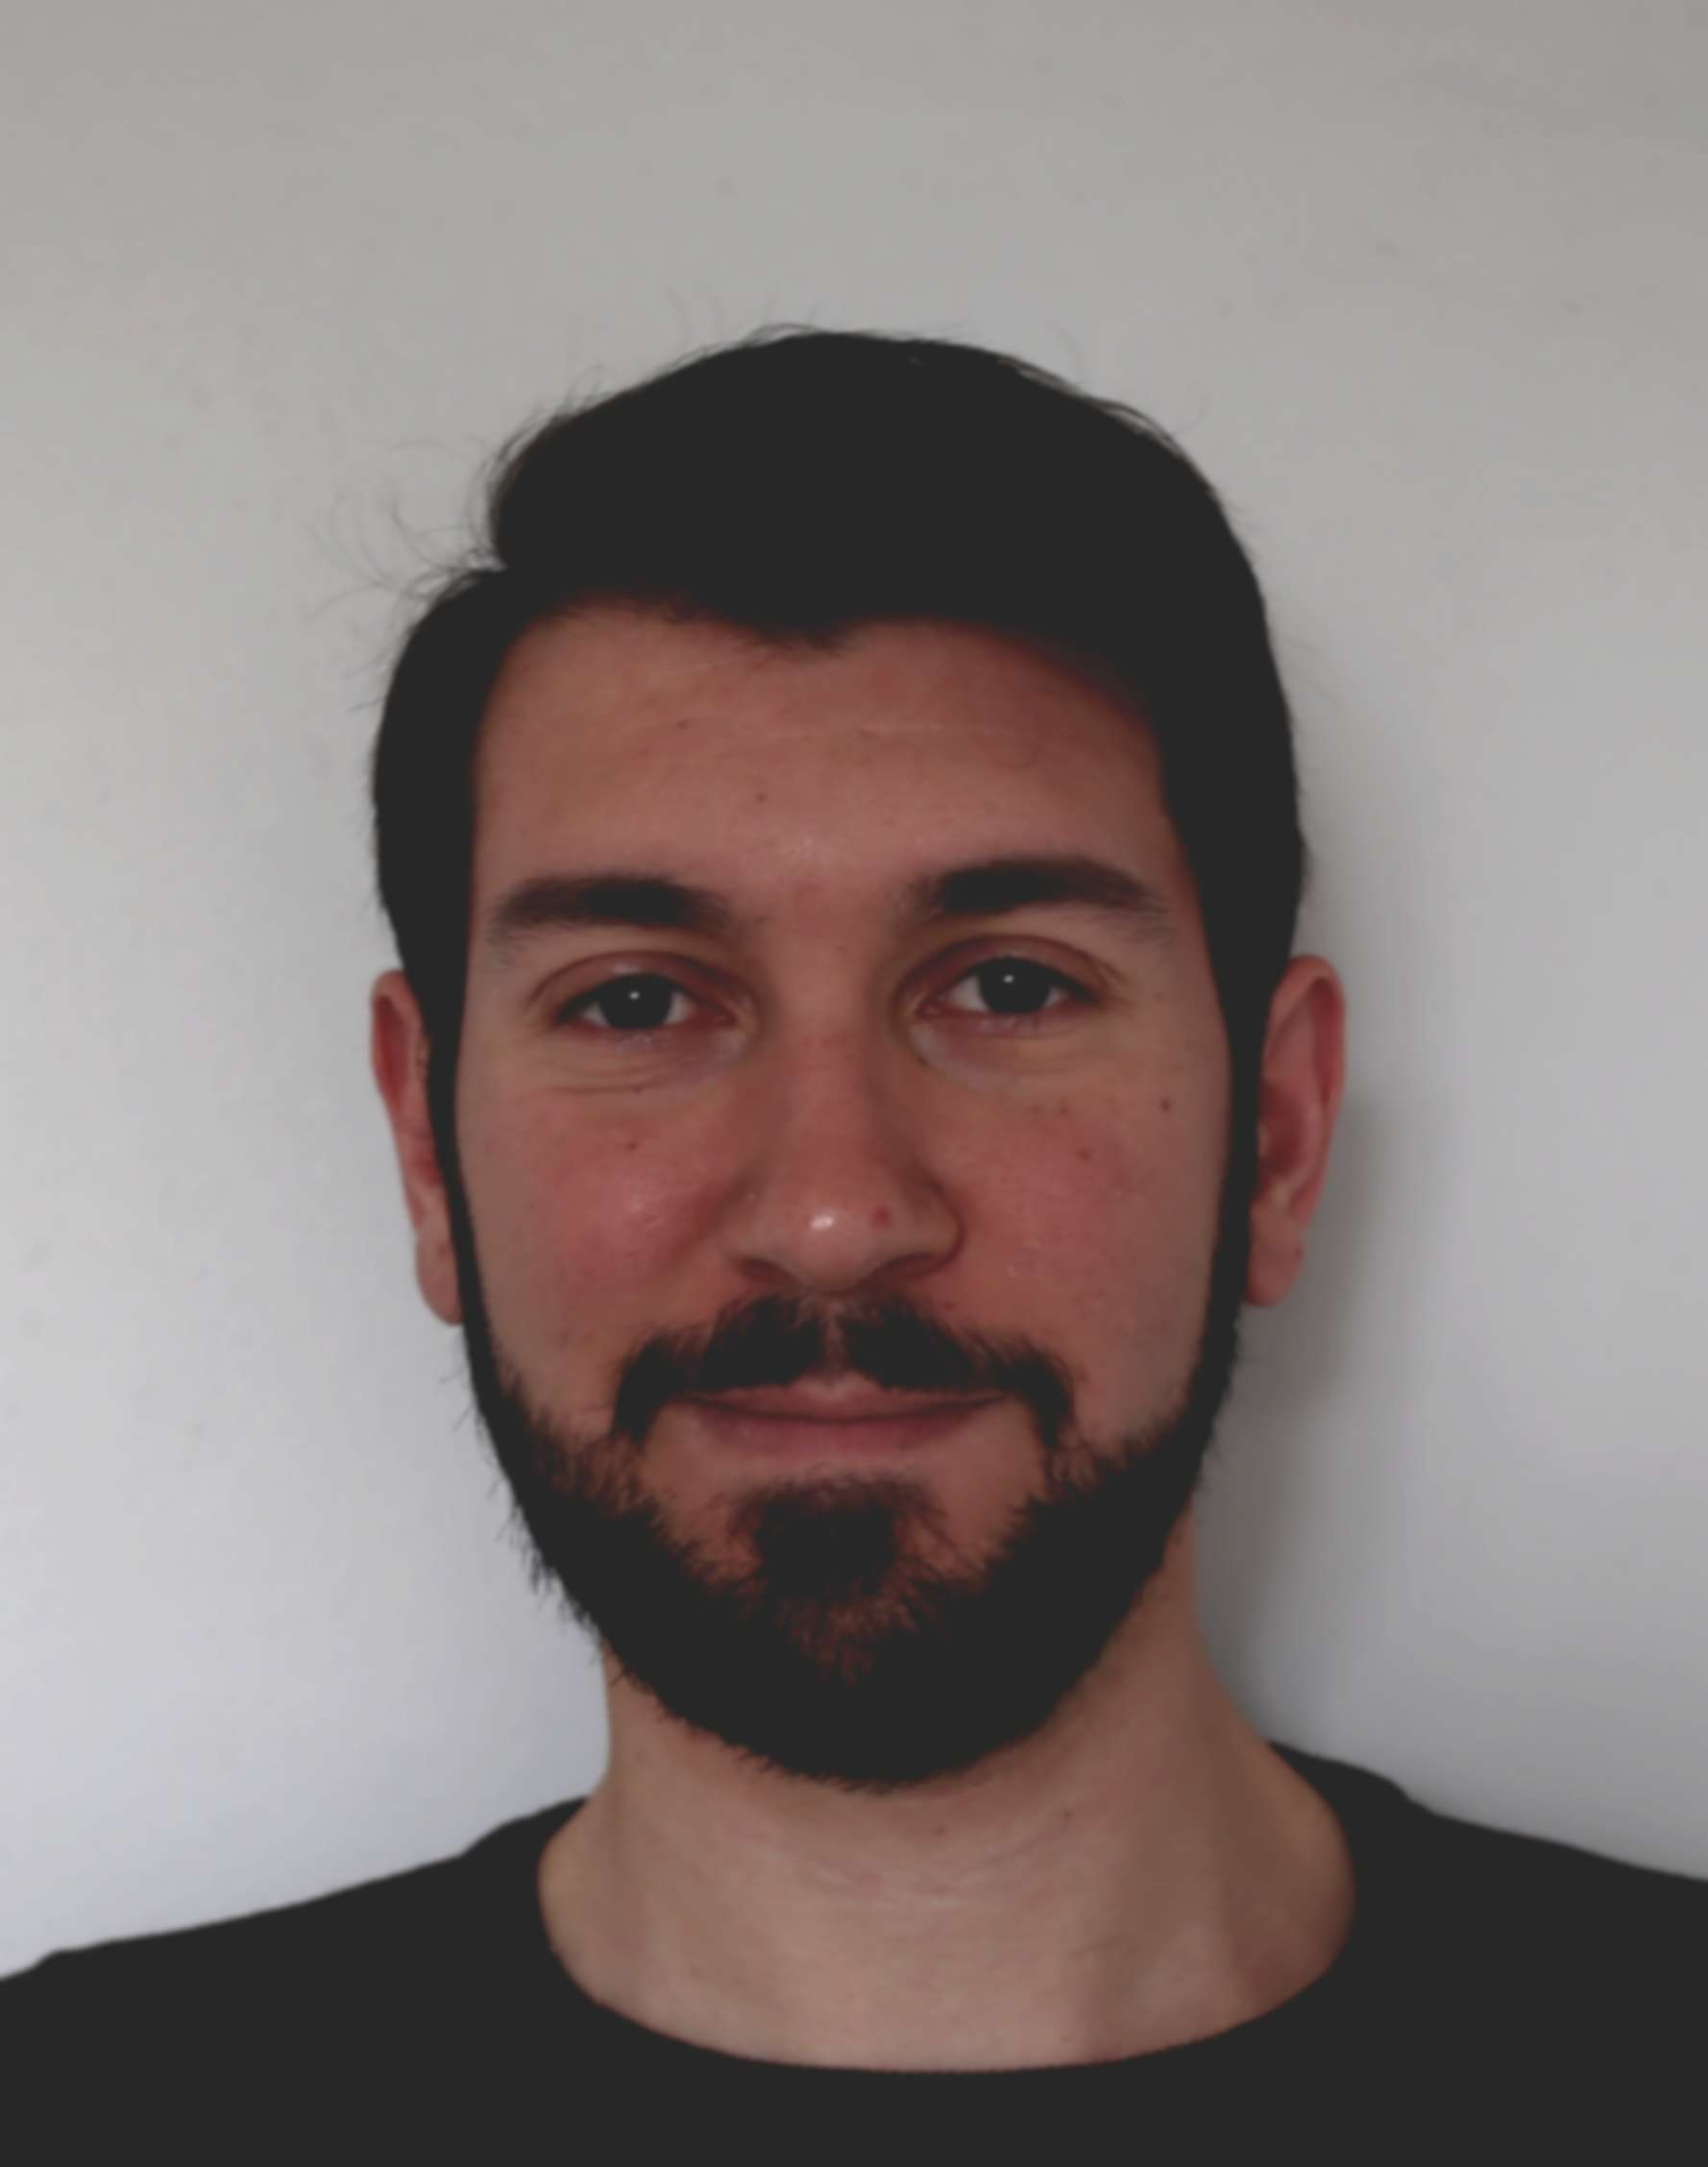
\includegraphics[width=0.6\textwidth]{IMG_2009.JPG}\\
31 Ans \\
Nationalité Italienne \\
Permis B \\
72 Quai de Tounis \\
31000 Toulouse - France \\
nicolaborghi@gmail.com \\
+33 (0)7 67 64 42 47 \\
LinkedIn://\href{https://www.linkedin.com/in/nicola-borghi/?locale=fr_FR}{nicola-borghi/} \\

%%%%%%%%%%%%%%%%%%%%%%%%%%%%%%%%%%%%%%
%     LINKS
%%%%%%%%%%%%%%%%%%%%%%%%%%%%%%%%%%%%%%

\section{Compétences}
\sectionsep
\location{Linguistiques}
%\vspace{\topsep} % Hacky fix for awkward extra vertical space
\vspace{1.2\topsep}
\begin{tightemize}
\item Italien - Langue maternelle
\item Français - C1
\item Anglais - C1
\end{tightemize}
\sectionsep
\location{Techniques}
%\vspace{\topsep} % Hacky fix for awkward extra vertical space
\begin{tightemize}
\item Définition des essais et développement des procédures
\item Préparation des essais et déroulement des opérations
\item Analyse des résultats d'essais
\item Définition des exigences du système
\item Gestion de projet et suivi du plan de développement
\end{tightemize}
\sectionsep
\location{Informatiques}
%\vspace{\topsep} % Hacky fix for awkward extra vertical space
\begin{tightemize}
\item Bus de données avioniques (MIL-STD-1553)
\item Programmation (Matlab, C\#, Python, LabView)
\item Rédaction de documentation (Office, Latex)
\item Gestion des exigences du système (IBM Rational DOORS)
\end{tightemize}
\sectionsep
\location{Sociales \& Communicationnelles}
%\vspace{\topsep} % Hacky fix for awkward extra vertical space
\begin{tightemize}
\vspace{\topsep}
Travail en équipe - Autonomie - Dynamisme
\end{tightemize}
\location{Centre d'interet}
%\vspace{\topsep} % Hacky fix for awkward extra vertical space
\begin{tightemize}
\vspace{\topsep}
Astronomie - Photographie numerique et argentique - Voyages
\end{tightemize}
%%%%%%%%%%%%%%%%%%%%%%%%%%%%%%%%%%%%%%
%
%     COLUMN TWO
%
%%%%%%%%%%%%%%%%%%%%%%%%%%%%%%%%%%%%%%
\end{minipage} 
\hfill
\begin{minipage}[t]{0.58\textwidth} 
%%%%%%%%%%%%%%%%%%%%%%%%%%%%%%%%%%%%%%
%     EDUCATION
%%%%%%%%%%%%%%%%%%%%%%%%%%%%%%%%%%%%%%
\hfill
\sectionsep

\section{Formation} 
\vspace{\topsep} % Hacky fix for awkward extra vertical space

\runsubsection{MASTER EN INGÉNIERIE SPATIALE}
\descript{\\ Sapienza - Università di Roma}
\location{Janvier 2011 - Janvier 2014 | Rome, IT}
\sectionsep

\runsubsection{Licence en ingénierie mécanique}
\descript{\\Università degli Studi di Ferrara}
\location{Octobre 2005 - Avril 2010 | Ferrara, IT}

\hfill

%%%%%%%%%%%%%%%%%%%%%%%%%%%%%%%%%%%%%%
%     EXPERIENCE
%%%%%%%%%%%%%%%%%%%%%%%%%%%%%%%%%%%%%%

\section{EXPÉRIENCES PROFESSIONNELLES}
\vspace{\topsep} % Hacky fix for awkward extra vertical space
\runsubsection{Thales Alenia Space}
\descript{| Consultant Ingénieur performance EGNOS }
\location{Juillet 2018 – Aujourd’hui | Toulouse, FR}
\begin{tightemize}
\item Évaluation des performance du système EGNOS V2 pendant les phases de qualification systeme (redaction de procedures de test,analyse des performance systeme et redactions des dossier de qualification) \\
\end{tightemize}
\sectionsep

\vspace{\topsep} % Hacky fix for awkward extra vertical space
\runsubsection{ELV / AVIO}
\descript{| Consultant Ingénieur système \& ingénieur de test }
\location{Juin 2016 – Juillet 2018 | Colleferro, IT}
\vspace{\topsep} % Hacky fix for awkward extra vertical space
\begin{tightemize}
\item Responsable Technique des sous-systèmes Thrust Vector Control (TVC) du lanceur VEGA : suivi du sous-traitant pendant la phase de production (participation aux TRR, TRB et DRB sous-système et résolution anomalies) \\
\item Responsable Technique des sous-systèmes Thrust Vector Control (TVC) du lanceur VEGA-C en développement : suivi de la phase de développement, préparation, déroulement et exploitation des essais système (e.g. essais à feu des moteurs Z40 et P120C)\\
\end{tightemize}
\sectionsep

\runsubsection{GMSpazio}
\descript{| Ingénieur modélisation et simulation \&
ingénieur système }
\location{Octobre 2014 - Juin 2016 | Rome, IT}
\vspace{\topsep} % Hacky fix for awkward extra vertical space
\begin{tightemize}
\item Ingénieur Système pour systèmes optiques pour le tracking de satellites et debris spatiaux  \\
\item Développeur de logiciels pour la simulation de missions spatiales \\
\item Formateur pour le logiciel AGI System ToolKit (STK) et Orbital Determination ToolKit (ODTK) \\
\end{tightemize}
\sectionsep

\runsubsection{Spacesys}
\descript{| Ingénieur Système}
\location{Avril 2014 - Octobre 2014 | Rome, IT}
\vspace{\topsep} % Hacky fix for awkward extra vertical space
\begin{tightemize}
\item Ingénieur Système pour le projet ESA Monav - Etude de fiabilité d’un système de navigation hybride GNSS/inertielle pour la navigation vers la Lune
\end{tightemize}
\sectionsep

\runsubsection{Thales Alenia Space}
\descript{| Étudiant Ingénieur Système}
\location{Juin 2013 – Décembre 2013 | Rome, IT}
\vspace{\topsep} % Hacky fix for awkward extra vertical space
\begin{tightemize}
\item Projet préliminaire d’un radar sondeur pour l’identification et la cartographie des cavités lunaires
\end{tightemize}
\sectionsep




\end{minipage} 
\end{document}  \documentclass[]{article}